\section{Modelos de neurônio de disparo}
\subsection{Leaky integrate-and-fire}
\begin{frame}{Circuito equivalente da membrana neuronal}
	\begin{columns}[t]
		\column{5cm}
			\begin{figure}[htb!]
				\centering
				\caption{Circuito equivalente da membrana}
				\label{fig:circuitomembrana}
				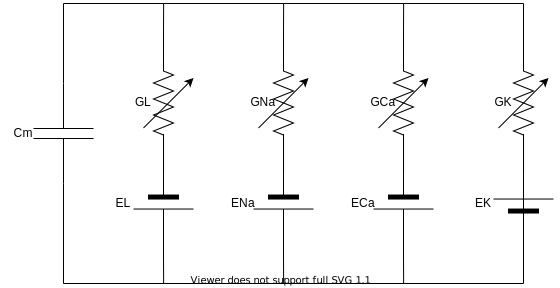
\includegraphics[width=\linewidth]{figs/circuito_membrana}
%				\fonte{O autor (\the\year)}
			\end{figure}
		\column{5cm}
			\begin{itemize}
				\item O capacitor está associado à capacitância de membrana;
				\item $G_L$ e $E_L$ referem-se aos elementos de vazamento;
				\item os demais são referentes aos canais iônicos dependentes de tensão.
				\note{na: sódio}
				\note{ca: cálcio}
				\note{k: potássio}
			\end{itemize}
	\end{columns}
	\vfill
	\[
		c_m\frac{\mathrm{d}V_m}{\mathrm{d}t}=G_{Na}(E_{Na}-V_m)+G_{Ca}(E_{Ca}-Vm)+G_K(E_K-V_m)+G_L(E_L-V_m)
	\]
\end{frame}

\begin{frame}{Modelo \textit{Leaky integrate-and-fire} (LIF)}
	\begin{columns}[t]
		\column{5cm}
			\begin{figure}[htb!]
				\centering
				\caption{Circuito equivalente do modelo LIF}
				\label{fig:circuitolif}
				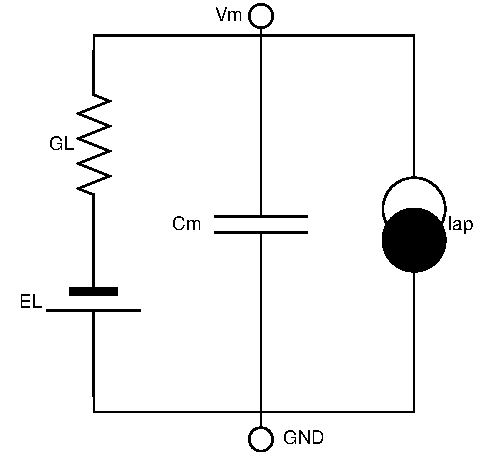
\includegraphics[width=0.5\linewidth]{figs/circuito_lif}
%				\fonte{O autor (\the\year)}
				%TODO: trocar GND
			\end{figure}
		\column{5cm}
			\begin{itemize}
				\item inclui uma corrente ($I_{ap}$) que é acumulada (integrada);
				\item contém uma condição que força o disparo (\textit{fire}) do potencial de ação no valor limite ($V_{th}$);
				\item no disparo, o potencial de membrana é atualizado para um valor de \textit{reset} ($V_{reset}$).
				\note{o modelo não representa a hiperpolarização que ocorre após o disparo, por isso o reset é acrescentado}
			\end{itemize}
	\end{columns}
	\vfill
	\[
		c_m\frac{dV_m}{dt} = G_L(E_L-V_m)+I_{ap}; \text{ se } V_m > V_{th} \text{ então } V_m\mapsto V_{reset}
	\]
\end{frame}

\begin{frame}{Modelo \textit{Leaky integrate-and-fire} (LIF)}
	\begin{figure}
		\centering
		\caption{Exemplo da simulação com o modelo LIF}
		\label{fig:lif}
		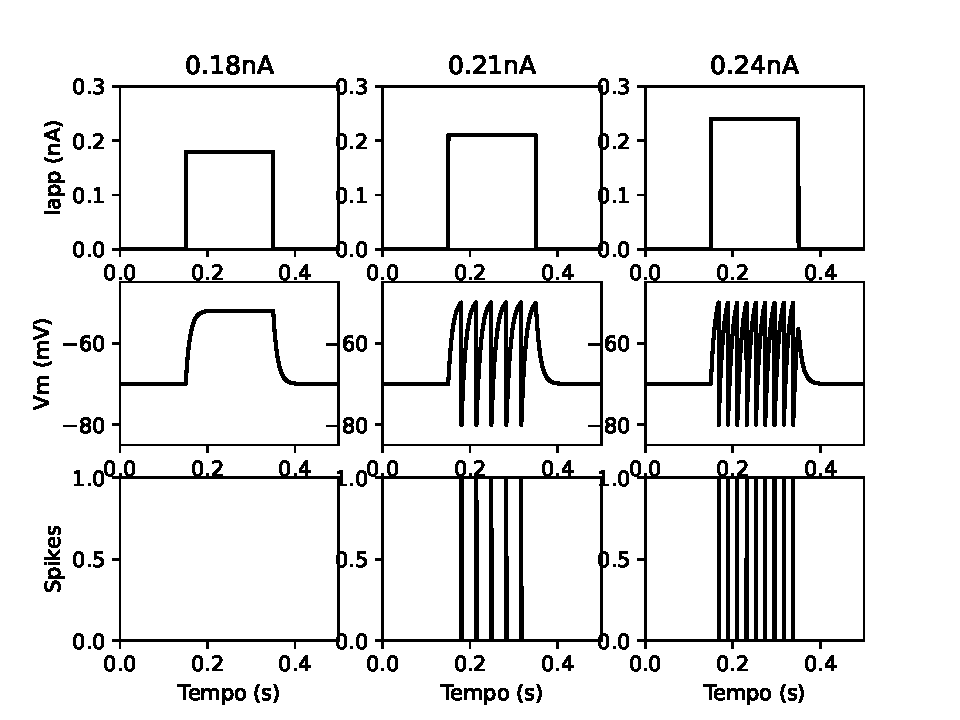
\includegraphics[width=0.5\linewidth]{figs/lif}
%		\fonte{O autor (\the\year)}
		%TODO: regerar
	\end{figure}
\end{frame}

\begin{frame}{Período refratário}
	\begin{columns}[t]
		\column{5cm}
			\begin{figure}
				\centering
				\caption{Simulação do modelo LIF com período refratário}
				\label{fig:lifrefratario}
				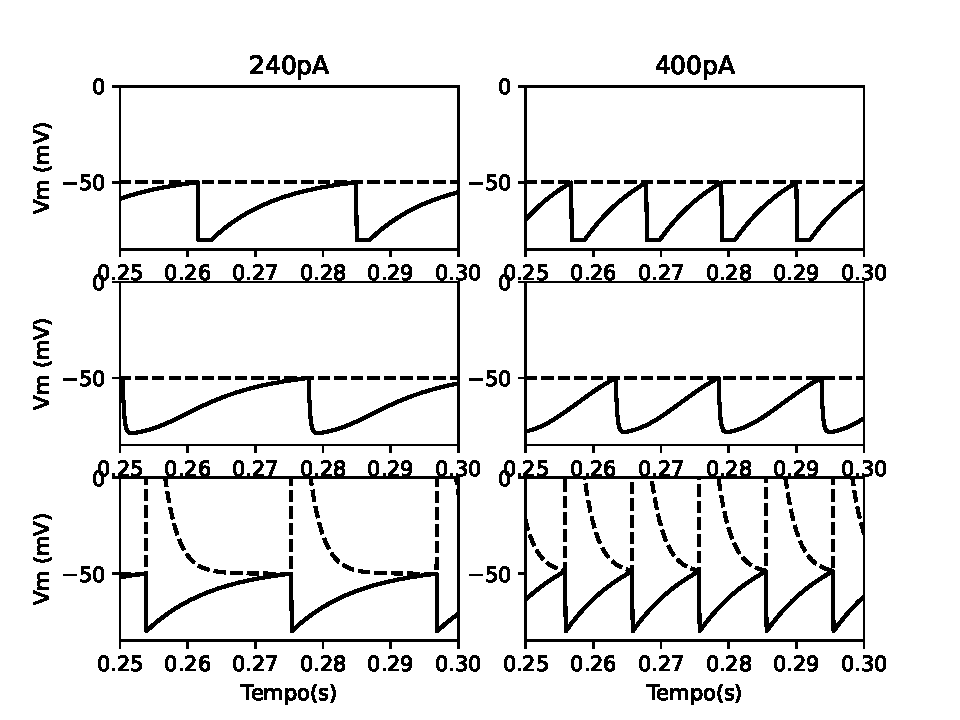
\includegraphics[width=\linewidth]{figs/lif_refratario}
%				\fonte{O autor (\the\year)}
				%TODO: regerar
			\end{figure}
		\column{5cm}
		\begin{itemize}
			\item intervalo de tempo que o neurônio não produz um novo disparo;
			\item não é presente no modelo LIF, por isso é acrescentado como extensão;
			\item métodos existentes para simular incluem o grampeamento de tensão, a condutância refratária e o incremento do limiar.
			\note{grampeamento de tensão: fixa o potencial de membrana no valor de reset}
			\note{condutância refratária: acrescenta uma condutância elevada, geralmente uma corrente hiperpolarizante de potássio, fazendo com que o potencial de membrana cresça em um ritmo mais lento}
			\note{incremento do limiar: aumenta o valor do limiar após cada potencial de ação}
		\end{itemize}
	\end{columns}
\end{frame}

\begin{frame}{Adaptação da taxa de disparos}
	\begin{columns}[t]
		\column{5cm}
			\begin{figure}
				\centering
				\caption{Adaptação da taxa de disparo no neurônio LIF}
				\label{fig:lifatd}
				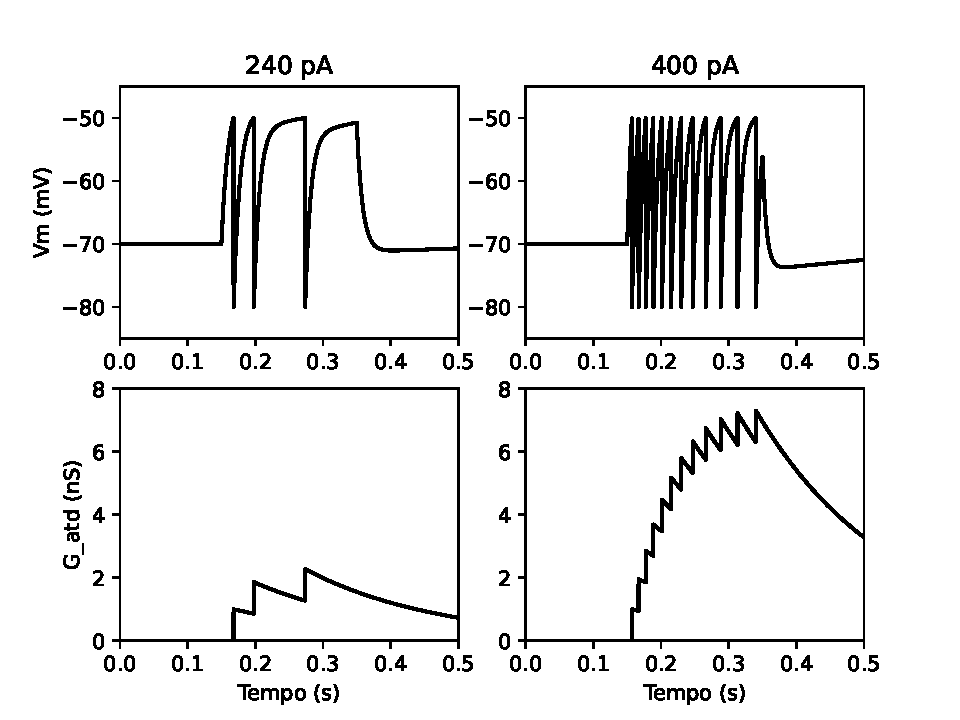
\includegraphics[width=\linewidth]{figs/lif_atd}
%				\fonte{O autor (\the\year)}
				%TODO: regerar
			\end{figure}
		\column{5cm}
		\begin{itemize}
			\item Diminuição da taxa de disparos logo após o primeiro; 
			\item é implementado de maneira semelhante ao método da condutância refratária;
			\item difere pelo valor do incremento de condutância, que é menor, e a escala de tempo, que é maior.
			\note{Uma fácil percepção da consequência da adaptação da taxa de disparo é a diferença de percepção de cheiros intensos ao longo do tempo, como quando uma pessoa entra com um perfume forte em um elevador}
			\note{o incremento menor não impede o disparo de novos potenciais, só diminui a taxa}
			\note{a escala de tempo maior permite o acúmulo das condutâncias ao longo da sequência de disparos}
		\end{itemize}
	\end{columns}
\end{frame}

\begin{frame}{Modelo \textit{Exponential leaky integrate-and-fire} (ELIF)}
	\begin{columns}[t]
		\column{5cm}
			\begin{figure}[tb]
				\centering
				\caption{Comparação dos modelos LIF e ELIF}
				\label{fig:elif}
				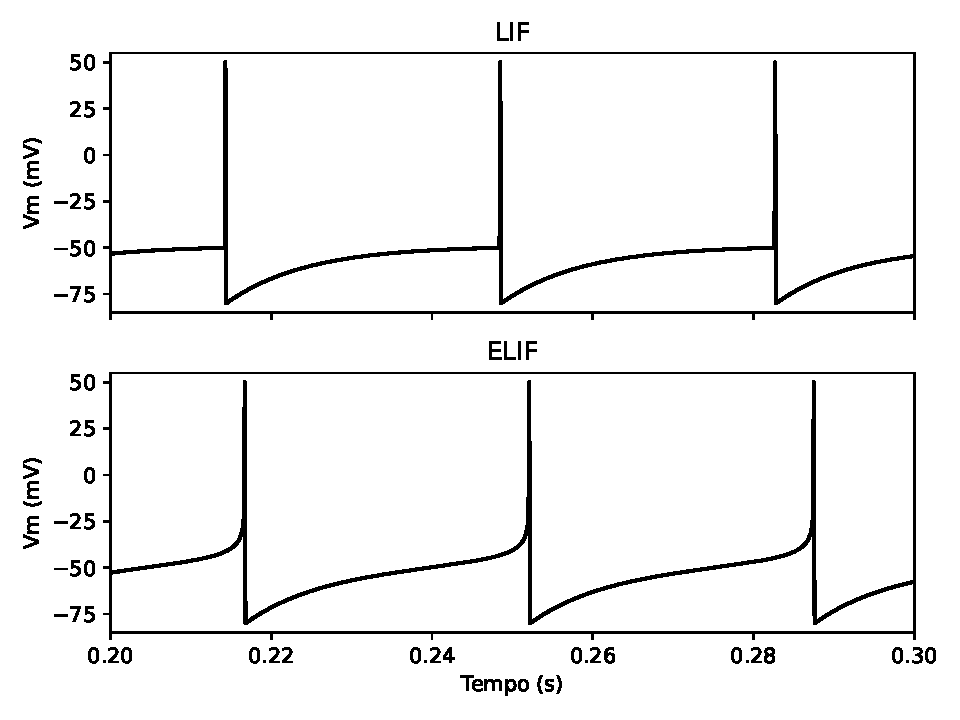
\includegraphics[width=0.8\linewidth]{figs/elif}
%				\fonte{O autor (\the\year)}
				%TODO: regerar
			\end{figure}
			\[
				\text{se } V_m > V_{max} \text{ então } V_m\mapsto V_{reset}
			\]
		\column{5cm}
		\begin{itemize}
			\item Incorpora um termo adicional para a geração do potencial de ação;
			\item acrescenta uma corrente despolarizante que eleva quase instantaneamente o valor do potencial de membrana;
			\item o crescimento tende ao infinito, mas é definido um limite nas simulações.
			\note{o computador tem problemas com valores infinitos, por isso o limite}
		\end{itemize}
	\end{columns}
	\vfill
	\[
	c_m\frac{dV_m}{dt} = G_L(E_L-V_m) + G_L\Delta_{th}\exp\Big(\frac{V_m-V_{th}}{\Delta_{th}}\Big) + I_{ap}
	\]
\end{frame}

\begin{frame}{Modelo \textit{Adaptative exponential leaky integrate-and-fire} (AELIF)}
	\begin{columns}[t]
		\column{5cm}
			\begin{figure}[tb]
				\centering
				\caption{Resposta do modelo AELIF}
				\label{fig:adexrs}
				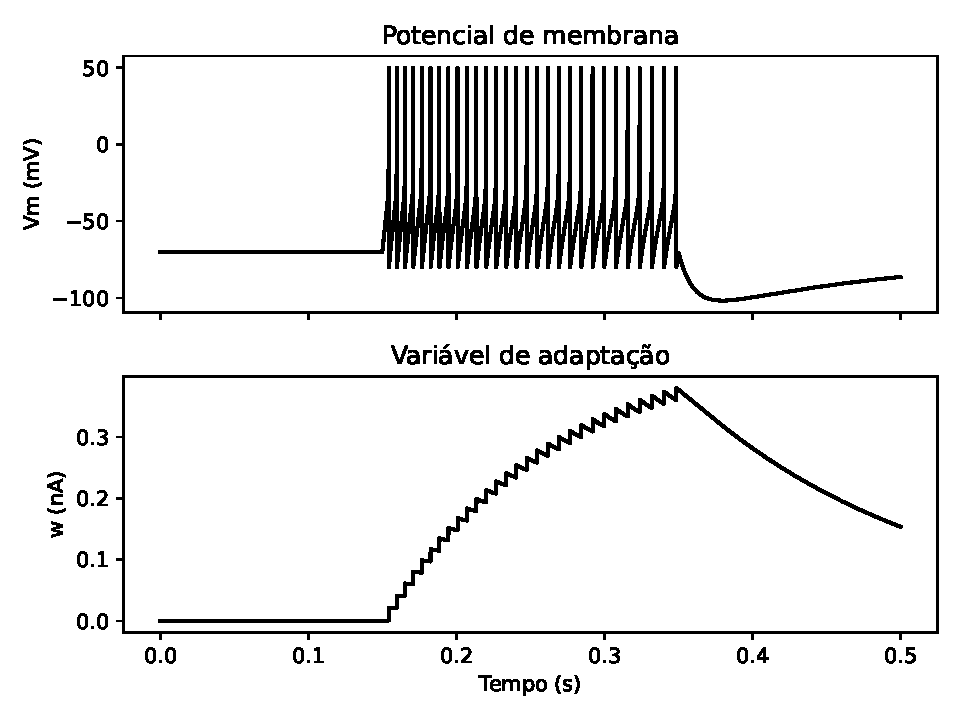
\includegraphics[width=0.8\linewidth]{figs/aelif}
%				\fonte{O autor (\the\year)}
				%TODO: regerar
			\end{figure}
			\note{Resposta do modelo AELIF para um pulso de corrente de 1 $nA$}
		\column{5cm}
		\begin{itemize}
			\item Adiciona uma corrente adaptativa hiperpolarizante;
			\item modelo de duas equações, para o potencial de membrana e a variável de adaptação ($w$).
			\note{a: parâmetro de agrupamento}
			\note{b: parâmetro de adaptação (incremento de corrente após o disparo)}
			\note{a curva de adaptação é semelhante à condutância adaptativa e condutância refratária}
		\end{itemize}
		\[
			\text{se } V_m > V_{max} \text{: } V_m\mapsto V_{reset} \text{ e } w\mapsto w + b
		\]
	\end{columns}
	\vfill
	\[
	c_m\frac{dV_m}{dt} = G_L(E_L-V_m) + G_L\Delta_{th}\exp\Big(\frac{V_m-V_{th}}{\Delta_{th}}\Big) - w + I_{ap}
	\]\[
	\tau_w\frac{dw}{dt}=a(V_m-E_L)-w
	\]
\end{frame}

\subsection{Izhikevich}

\subsection{Hodgkin-Huxley}
